%
% RFBA.tex
% Main LaTeX document for formatting RFBA
%
% R for Business Administration
%
% Copyright (C) 2016 Harris Kenny, Brandon DeGolier, Nate Lewis
%
% This document is licensed under the Creative Commons Attribution 4.0
% International Public License (CC BY-SA 4.0)
%

%%% XXX NOTE

%%% Glossaries and indices are broken:
%%% https://sharelatex.tenderapp.com/help/discussions/questions/19378-glossaries-indices-and-speed

%%% XXX NOTE


% LaTeX Docs:
% http://en.wikibooks.org/wiki/Category:LaTeX

% LaTeX Memoir Class
% Docs: /usr/share/doc/texlive-latex-recommended-doc/latex/memoir/memman.pdf
\documentclass[twoside,12pt,openright,final,english]{memoir}


\usepackage{tikz}
\usetikzlibrary{shadows,shapes,arrows,chains,calc,decorations.pathmorphing,patterns,trees,positioning,automata,fit}
% This breaks things, but would be great to use
%\usepackage{tikz-qtree,tikz-qtree-compat}
\usepackage{rotating}
\usepackage{forest}

\usetikzlibrary{arrows,shapes}
\usetikzlibrary{positioning,calendar,er}
\usetikzlibrary{decorations.markings}
\usetikzlibrary{shapes.geometric}


\usepackage{smartdiagram}
\usesmartdiagramlibrary{additions}
\usepackage{comment}  % Padding? /usr/share/doc/texlive-doc/latex/comment/comment.pdf
\usepackage{graphicx} % Docs: /usr/share/doc/texlive-doc/latex/graphics/graphicx.pdf
\usepackage{epstopdf} % Docs: /usr/share/doc/texlive-doc/latex/oberdiek/epstopdf.pdf
\usepackage[colorlinks=true]{hyperref}
    % Docs: http://en.wikibooks.org/wiki/LaTeX/Hyperlinks
    %       http://www.tug.org/applications/hyperref/manual.html
\graphicspath{{./images/}}

\makeindex
\makeglossary

\usepackage{color} % Docs: /usr/share/doc/texlive-latex-base-doc/latex/graphics/grfguide.pdf
%\usepackage[usenames,dvipsnames,svgnames,table]{xcolor}

%%% PREAMBLE FONTS %%%
% For XeTeX
% http://www.ctan.org/pkg/fontspec
% http://mirrors.ctan.org/macros/latex/contrib/fontspec/fontspec.pdf
\usepackage{fontspec}
\defaultfontfeatures{Ligatures=TeX} % To support LaTeX quoting style
\setmainfont{lmroman12-regular.otf}

\usepackage[normalem]{ulem} % underline

\usepackage{floatpag} % Full page figures without page numbers.

%%% END PREAMBLE FONTS %%%

%%% PAGE, STOCK, AND MARGIN SIZE %%%
% 7.44 x 9.68"   18.90 x 24.58cm
\setstocksize{24.58cm}{18.90cm} % { height }{ width }
\settrimmedsize{\stockheight}{\stockwidth}{*}

%\settypeblocksize{ height }{ width }{ ratio }
\settypeblocksize{19.0cm}{*}{*}

%\setlrmarginsandblock{ spine }{ edge }{ ratio }
% make the spine have more space than outer edge
\setlrmarginsandblock{*}{2.5cm}{1.2}

% \setulmargins{ upper }{ lower }{ ratio }
\setulmargins{2.0cm}{*}{*}

% \setheadfoot{ headheight }{ footskip }
\setheadfoot{12pt}{2cm}

\checkandfixthelayout[fixed]
%%% END PAGE, STOCK, AND MARGIN SIZE %%%

\setcounter{secnumdepth}{3}
\setcounter{tocdepth}{3}

\usepackage[english]{babel}
\usepackage{datetime} % Docs: /usr/share/doc/texlive-doc/latex/datetime/datetime.pdf
\usepackage{ucs}

%%% PDFLATEX %%%
\usepackage{etex}

%%% Not all features are used in XeTeX
\usepackage[protrusion,babel,final]{microtype}
%%% Conflicts with package fontspec
%\usepackage[utf8x]{inputenc}

% Docs: /usr/share/doc/texlive-humanities-doc/latex/ledmac/ledmac.pdf
%\usepackage{eledmac}

%%% AOOM PAGE STYLE %%%
\makepagestyle{aoomstyle}
\pagestyle{aoomstyle}
\makeevenhead{aoomstyle}{}{\hspace{2em}\itshape\small\leftmark}{}
\makeoddhead{aoomstyle}{}{\scshape\small\rightmark}{}
\makeevenfoot{aoomstyle}{}{\hspace{2em}\thepage}{}
\makeoddfoot{aoomstyle}{}{\thepage}{}
%%% END AOOM PAGE STYLE %%%

%%% AOOMSKI CHAPTER STYLE %%%
\makechapterstyle{aoomski}{%
  \renewcommand*{\printchaptername}{}	% Clear out the chapter name (e.g. capítulo)
  \renewcommand*{\printchapternum}{}	% Clear out the chapter number
  \renewcommand*{\chaptitlefont}{\fontspec{Montserrat-Regular.ttf}\fontsize{20pt}{3em}\selectfont}	% Set chapter title font
  \renewcommand*{\printchaptertitle}[1]{%
     \hrule\vskip\onelineskip \centering \chaptitlefont{##1}\par}
  % Set chapter title font
  \renewcommand*{\afterchaptertitle}{\vskip\onelineskip \hrule\vskip
     \afterchapskip}
}
%%% END AOOMSKI CHAPTER STYLE %%%

%%% FORMATTING... %%%
\midsloppy
\setlength{\emergencystretch}{3em}
\tolerance=5000
\hyphenpenalty=500
\setlength{\topskip}{1.6\topskip}
\checkandfixthelayout
\raggedbottom
\widowpenalty=10000
\clubpenalty=10000
%%% END FORMATTING... %%%

%%% FOOTNOTES %%%
% no horizontal rule before footnotes:
\let\oldfootnoterule\footnoterule
\renewcommand*{\footnoterule}{}
\setlength{\footmarkwidth}{3.5em}
%%% END FOOTNOTES %%%

%%% COLORS %%%
\definecolor{ao-purple}{cmyk}{0.50,0.60,0.00,0.43}  % ???
%\definecolor{ao-purple}{cmyk}{0.85 0.90 0.00 0.05} % ???
\definecolor{ao-dark-blue}{cmyk}{0.83 0.24 0.00 0.12}
\definecolor{ao-light-blue}{cmyk}{0.41 0.15 0.00 0.09}
\definecolor{ao-light-orange}{cmyk}{0.00 0.40 0.88 0.03}
\definecolor{ao-dark-orange}{cmyk}{0.00 0.51 0.83 0.11}
\definecolor{ao-gold}{cmyk}{0.00 0.18 0.75 0.00}
\definecolor{ao-greyblack}{cmyk}{0.00 0.11 0.09 0.86}
\definecolor{ao-white}{cmyk}{0.00 0.00 0.00 0.00}
\definecolor{ao-black}{cmyk}{1.00 1.00 1.00 1.00}
\definecolor{lulzbot-green}{cmyk}{0.11 0.00 0.78 0.15}
%%% END COLORS %%%


%%% DEBUG %%%
%\showoutput
%\typeoutlayout
%\typeoutstandardlayout
%%% END DEBUG %%%

%%% END OF PREAMBLE %%%

\begin{document}

%%% BEGIN FRONT MATTER %%%
\frontmatter

% Set page numbers to lowercase roman numerals, and reset the count to 1 (no *)
\pagenumbering{roman}

%%% TITLE PAGE %%%
% We want the title to be on the right hand page.
% If we pad a page, it gives us two with openright
%
% Title.tex
%
% Aleph Objects Operations Manual
%
% Copyright (C) 2016, 2017 Harris Kenny, Brandon DeGolier, Nate Lewis
% Copyright (C) 2014, 2015 Aleph Objects, Inc.
%
% This document is licensed under the Creative Commons Attribution 4.0
% International Public License (CC BY-SA 4.0) by Aleph Objects, Inc.
%

\date {}
\thispagestyle{empty}
\begin{center}
\par
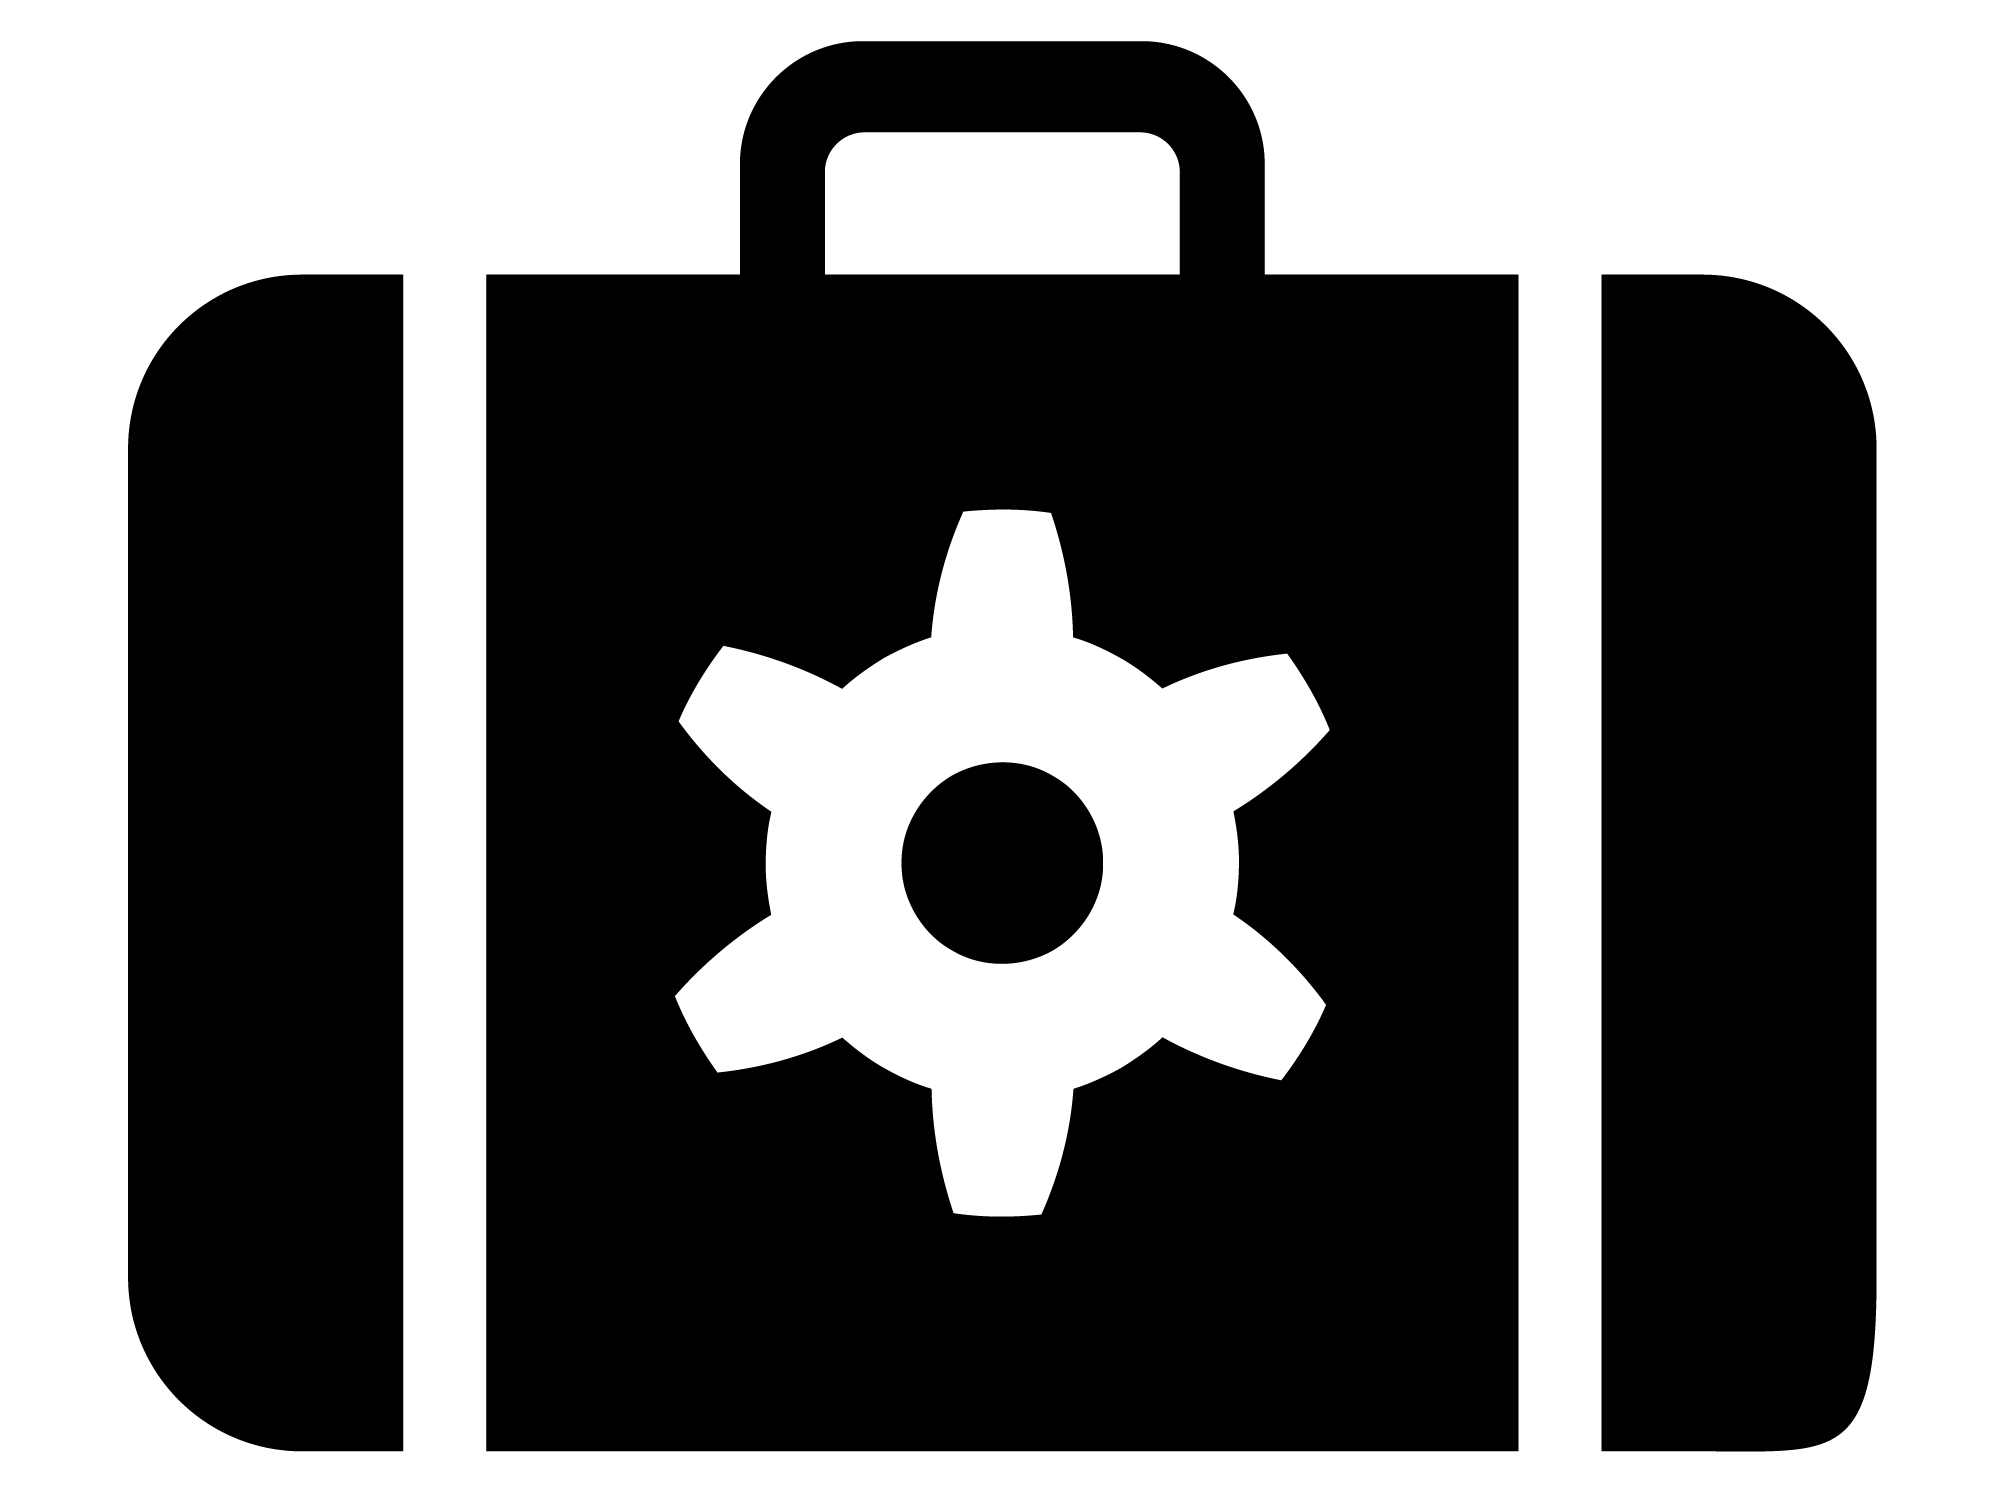
\includegraphics[keepaspectratio=true,angle=0,height=0.5\textheight,width=0.5\textwidth]{logobridge-briefcase.png}
\par
\null\vfill
{\fontspec{Outage.ttf}\fontsize{25pt}{5cm}\selectfont \textcolor{ao-purple}{R for Business Administration}}
\end{center}

%%% END TITLE PAGE

%%% COPYRIGHT PAGE %%%
%
% Copyright.tex
% Copyleft
%
% R for Business Administration
%
% Copyright (C) 2016 Harris Kenny, Brandon DeGolier, Nate Lewis
%
% This document is licensed under the Creative Commons Attribution 4.0
% International Public License (CC BY-SA 4.0)
%
\fontspec{Montserrat-Regular.ttf}

\clearpage\null\vfill
\begingroup 
\thispagestyle{empty}
\footnotesize\raggedright
\setlength{\parskip}{0.5\baselineskip}

\textbf{R for Business Administration}

Copyright \copyright\ \the\year\ Harris Kenny, Brandon DeGolier, Nate Lewis\par
Permission is granted to copy, distribute and\slash or modify 
this document under the terms of the
Creative Commons Attribution 4.0 International Public License
(CC BY-SA 4.0).

This work is derived from Aleph Objects Operations Manual (AOOM) by 
Aleph Objects, Inc. and shared under the terms of the 
Creative Commons Attribution 4.0 International Public License 
(CC BY-SA 4.0). For more information, visit: \texttt{https://alephobjects.com/}

R software and documentation is held and administered by the R
Foundation, a not for profit organization working in the public interest.
Learn more online: \texttt{https://www.r-project.org/foundation/}

% ISBN: NNN-N-NNN-NNNNN-N
\renewcommand{\dateseparator}{}
\hfill\texttt{\yyyymmdddate\today} % Timestamp build date
\endgroup
\pagebreak{}


%%% END COPYRIGHT PAGE %%%

%%% ACKNOWLEDGMENT PAGE %%%
%
% Copyright.tex
% Acknowledgment
%
% R for Business Administration
%
% Copyright (C) 2016 Harris Kenny, Brandon DeGolier, Nate Lewis
%
% This document is licensed under the Creative Commons Attribution 4.0
% International Public License (CC BY-SA 4.0)
%

\section{Acknowledgment}

Special thanks to Dr. Anthony Hayter, who encouraged and supported the 
original authors of this work to use R in his Professional Master of 
Business Administration Statistics course (STAT 4610-17) at the 
University of Denver Daniels College of Business in Denver, Colorado, 
USA in Spring 2016.
%%% END ACKNOWLEDGMENT PAGE %%%

%%% TABLE OF CONTENTS %%%
{\fontspec{Montserrat-Regular.ttf}
\maxtocdepth{section}
\settocdepth{section}
% space between dots
\renewcommand{\cftchapterdotsep}{15}
% dot symbol (default is period)
\renewcommand{\cftdot}{\textperiodcentered}	% centered period
% Set space between each entry in ToC
\setlength{\cftbeforechapterskip}{5pt}
\tableofcontents*}
%%% END TABLE OF CONTENTS %%%

%%% LIST OF FIGURES %%%
\renewcommand*{\lofheadstart}{\vspace{1cm}}
\clearpage
\listoffigures*
%%% END LIST OF FIGURES %%%

%%% CHAPTER STYLE %%%
\chapterstyle{aoomski} % defined in preamble
\def\topblockvspace{0.11}
%%% END CHAPTER STYLE %%%

%%% CHAPTER CONFIG %%%
\newcommand{\chapterheader}{R for Business Administration}
% See \chapterconf below for examples of how this is used.
% value 1 is file to include
% value 2 is title of chapter
% value 3 is sub title of chapter
\newcommand{\chapterconf}[3]{
\chapter{\emph{{#2}}\protect \\
{#3}}
\thispagestyle{empty}
\markboth{#2}{\chapterheader}
{\include{#1}}
}
%%% END CHAPTER CONFIG %%%

%%% FRONTMATTER CHAPTERS %%%
\fontspec{lmroman12-regular.otf}

% Format:
% \chapterconf{Name of file to include}{Title of Chapter}
%%% END FRONTMATTER CHAPTERS %%%
\chapterconf{Introduction}{Introduction}{Purpose of this Work}
%%% END FRONTMATTER %%%

%%% BEGIN MAINMATTER %%%
\mainmatter*

% Set page numbering to arabic, but don't reset numbering (*)
\pagenumbering*{arabic}

%% MAINMATTER CHAPTERS %%%
% Default chapter font
\fontspec{lmroman12-regular.otf}

% Format:
% \chapterconf{Name of file to include}{Title of Chapter}{Subtitle}
% Comment out a line to not render that chapter
\chapterconf{Installation}{Installation}{Getting Ready}
\chapterconf{Basics}{Basics}{Getting Started}
\chapterconf{Surveys}{Surveys}{Understanding Collected Data}
\chapterconf{Contact}{Contact}{Getting in Touch}

%\chapterconf{Sample}{{\LaTeX} Samples}{Snippets here}
%% END MAINMATTER CHAPTERS %%%

%%% END MAINMATTER %%%

%%% BEGIN BACKMATTER %%%
\backmatter

%%% INDEX %%%
% \clearpage
\printindex
%%% END INDEX %%%

%%% GLOSSARY %%%
\renewcommand{\memgloterm}[1]{\textbf{#1}}
\renewcommand{\memglodesc}[1]{\textit{#1}}
\renewcommand{\memglonum}[1]{}

% \clearpage
\printglossary
%%% END GLOSSARY %%%

%%% COLOPHON %%%
%%% skip a couple pages
\pagebreak{}
\thispagestyle{empty}
\begingroup 
\vfill\null 
\endgroup
\pagebreak{}
\thispagestyle{empty}
\fontspec{Montserrat-Regular.ttf}
{%
% Colophon.tex
%
% Aleph Objects Operations Manual
%
% Copyright (C) 2014, 2015 Aleph Objects, Inc.
%
% This document is licensed under the Creative Commons Attribution 4.0
% International Public License (CC BY-SA 4.0) by Aleph Objects, Inc.
%

%%% COLOPHON %%%
\begin{vplace}
\centering
\emph{\LARGE Colophon}

\rule{0.5\textwidth}{0.4pt}\\[\baselineskip]

{\tiny Created with 100\% Free Software}

GNU/Linux

{\LaTeX} Memoir

\rule{0\textwidth}{0pt}\\[\baselineskip]%
\rule{0.5\textwidth}{0.4pt}\\[\baselineskip]
\end{vplace}
%%% END COLOPHON %%%

}
%%% END COLOPHON %%%

%%% END BACKMATTER %%%

\end{document}
